%!TEX root = thesis.tex

\chapter{COMBINING ILLUMINATION INVARIANCE WITH OCCLUSION ROBUSTNESS, AND ALIGNMENT}
\label{chap:cvpr}

%\documentclass[10pt,twocolumn,letterpaper]{article}

%\usepackage{cvpr}
%\usepackage{times}
%\usepackage{epsfig}
%\usepackage{graphicx}
%\usepackage{amsmath}
%\usepackage{amsfonts}
%\usepackage{amscd}
%\usepackage{amssymb}
%\usepackage{subfigure}
%\usepackage{pdfsync}
%\usepackage{helvet}
%\usepackage{url}

%% Include other packages here, before hyperref.
%\usepackage{mydefs}
%\usepackage{algorithm}
%\usepackage{algorithmic}

%\newcommand{\jw}[1]{{\bf \textcolor{blue}{John: #1}}}
%%\newcommand{\aw}[1]{\bf \color{greem} Drew: #1}
%%\newcommand{\ym}[1]{\bf \color{red}{ Yi: #1}}

%% If you comment hyperref and then uncomment it, you should delete
%% egpaper.aux before re-running latex.  (Or just hit 'q' on the first latex
%% run, let it finish, and you should be clear).
%%\usepackage[pagebackref=true,breaklinks=true,letterpaper=true,colorlinks,bookmarks=false]{hyperref}

%
% \cvprfinalcopy % *** Uncomment this line for the final submission

%\def\cvprPaperID{1291} % *** Enter the CVPR Paper ID here
%\def\httilde{\mbox{\tt\raisebox{-.5ex}{\symbol{126}}}}

%% Pages are numbered in submission mode, and unnumbered in camera-ready
%\ifcvprfinal\pagestyle{empty}\fi
%\begin{document}

%%%%%%%%%% TITLE
%\title{Towards a Practical Face Recognition System: \\ Robust Registration and
%Illumination by Sparse Representation\vspace{0mm}}

%\author{Andrew Wagner, John Wright, Arvind Ganesh, Zihan Zhou, Yi Ma\\
%University of Illinois at Urbana-Champaign, 1308 W. Main st. Urbana, IL 61801\\
%{\tt\small \{awagner, jnwright, abalasu2, zzhou7, yima\}@illinois.edu}}

%\maketitle
%% \thispagestyle{empty}

%%%%%%%%%% ABSTRACT
%\begin{abstract}\vspace{0mm}
%Most contemporary face recognition algorithms work well under
%laboratory conditions but degrade when tested in less-controlled environments. This is mostly due to the difficulty of simultaneously 
%handling variations in illumination, alignment, pose, and occlusion.
%In this paper, we propose a simple and practical  face recognition system that achieves a high degree of  
%robustness and stability to all these variations. We demonstrate how to use tools from sparse representation 
%to align a test face image with a set of frontal training 
%images in the presence of significant registration error and occlusion. We thoroughly characterize the region 
%of attraction for our alignment algorithm on public face datasets such as Multi-PIE. 
%We further study how to obtain a sufficient set of training illuminations for linearly  
%interpolating practical lighting conditions. We have implemented a complete face recognition
%system, including a projector-based training acquisition system, in order to evaluate how our algorithms work under practical testing conditions. We show  
%that our system can efficiently and effectively recognize faces under  
%a variety of realistic conditions, using only 
%frontal images under the proposed illuminations as training.\vspace{0mm}
%\end{abstract}

%%%%%%%%% BODY TEXT
\section{Introduction}\vspace{0mm}
%Automatic face recognition remains one of the most active areas in computer vision. 

This chapter represents work that I have performed in collaboration with John Wright,  Arvind Ganesh, Zihan Zhou, and Yi Ma.  It is an extended version of a conference paper that has been accepted for publication at the 2009 IEEE Conference on Computer Vision \cite{Wagner2009-CVPR}.  
There is a historical tendency for face recognition algorithms to work well under laboratory conditions but degrade when tested in less-controlled environments.  
Particularly in the few years following the attack on the World Trade Center in 2001, there have been several high profile failed trials of face recognition technology for security in the public sector.
This is mostly due to the difficulty of simultaneously handling variations in illumination, alignment, pose, and occlusion.
This chapter proposes a simple and practical  face recognition system that achieves a high degree of  
robustness and stability to all these variations. A technique for using tools from sparse representation 
to align a test face image with a set of frontal training 
images in the presence of significant registration error and occlusion is presented. The region 
of attraction of the alignment algorithm is thoroughly characterized on public face datasets such as Multi-PIE.
It is shown how to choose a sufficient set of training illuminations for linearly  
interpolating practical lighting conditions.  We have implemented a complete face recognition
system, including a projector-based training acquisition system, in order to evaluate how our algorithms work under practical testing conditions.  It is demonstrated  
that our system can efficiently and effectively recognize faces under  
a variety of realistic conditions, using only 
frontal images under the proposed illuminations as training.\vspace{0mm}

While classical algorithms \cite{Turk1991-CVPR,Belhumeur1997-PAMI} remain popular for their speed and simplicity, they tend to fail on large-scale, practical tests, falling short of the ultimate goal of truly automating face recognition for real-world applications such as access control for facilities, computer systems and automatic teller machines.  These application domains are interesting both for their potential sociological impact and also because they allow the possibility of carefully controlling the acquisition of the training data.  This allows for more tractable and reliable solutions that achieve higher recognition rates.\footnote{Face recognition with less-controlled training samples taken under uncontrolled scenarios remains an active research area as well \cite{LFW}.} In this setting, one promising recent direction, set forth in \cite{Wright2009-PAMI}, casts the recognition problem as one of finding a sparse representation of the test image in terms of the training set as a whole, up to some sparse error due to occlusion. 

\begin{figure}
\centering
\begin{tabular}{cc}
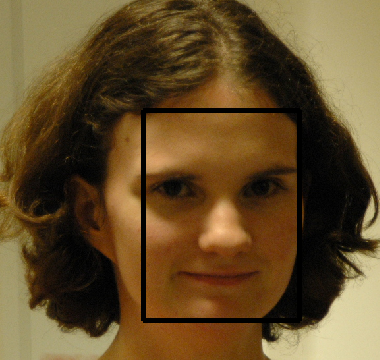
\includegraphics[height=1.2in]{figures_cvpr/promo/case1/detector.png}& \hspace{3mm}
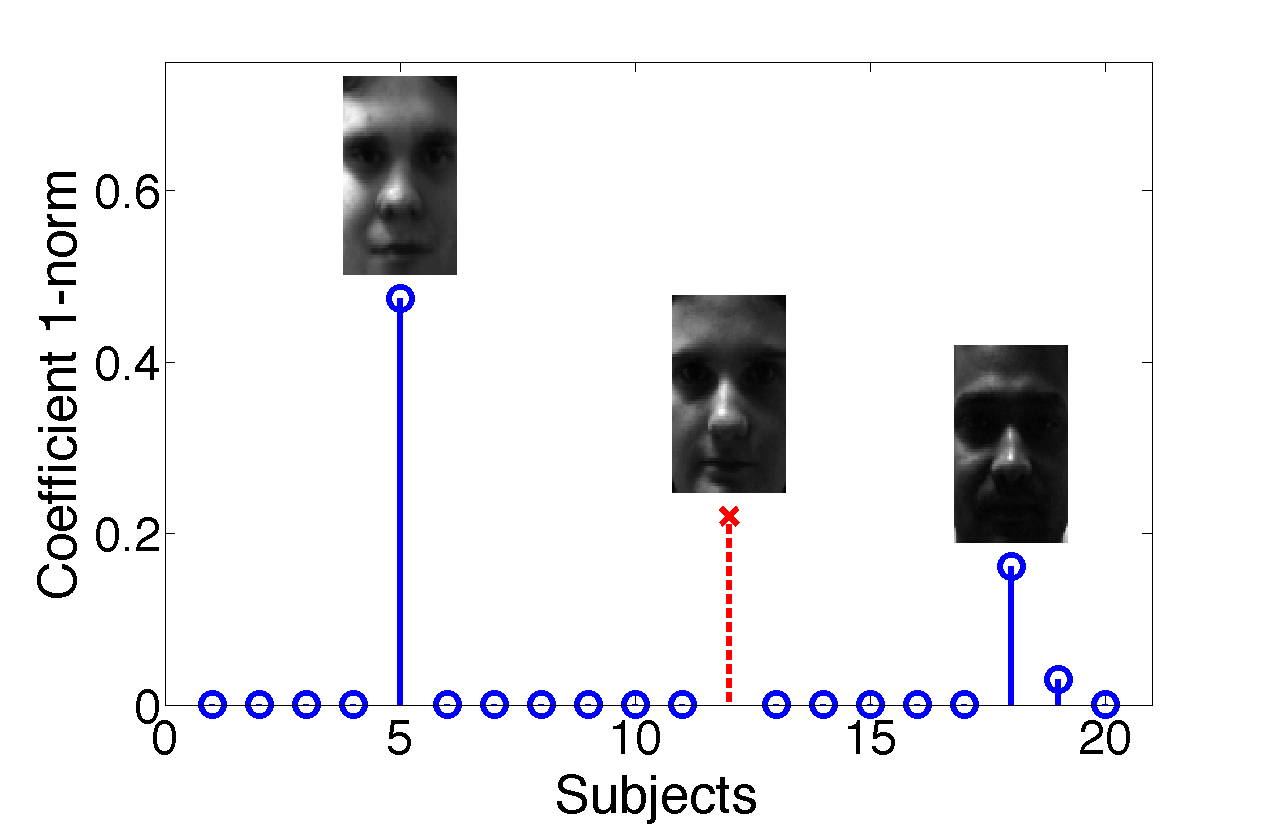
\includegraphics[height=1.2in]{figures_cvpr/promo/case1/sci_with_axis_face_case1.png} \\
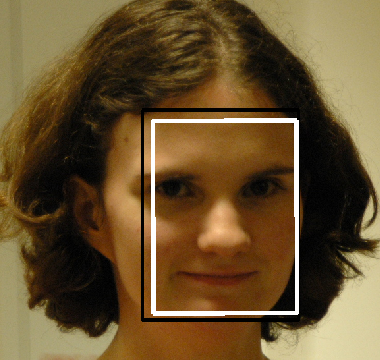
\includegraphics[height=1.2in]{figures_cvpr/promo/alignment_and_detector.png}& \hspace{3mm}
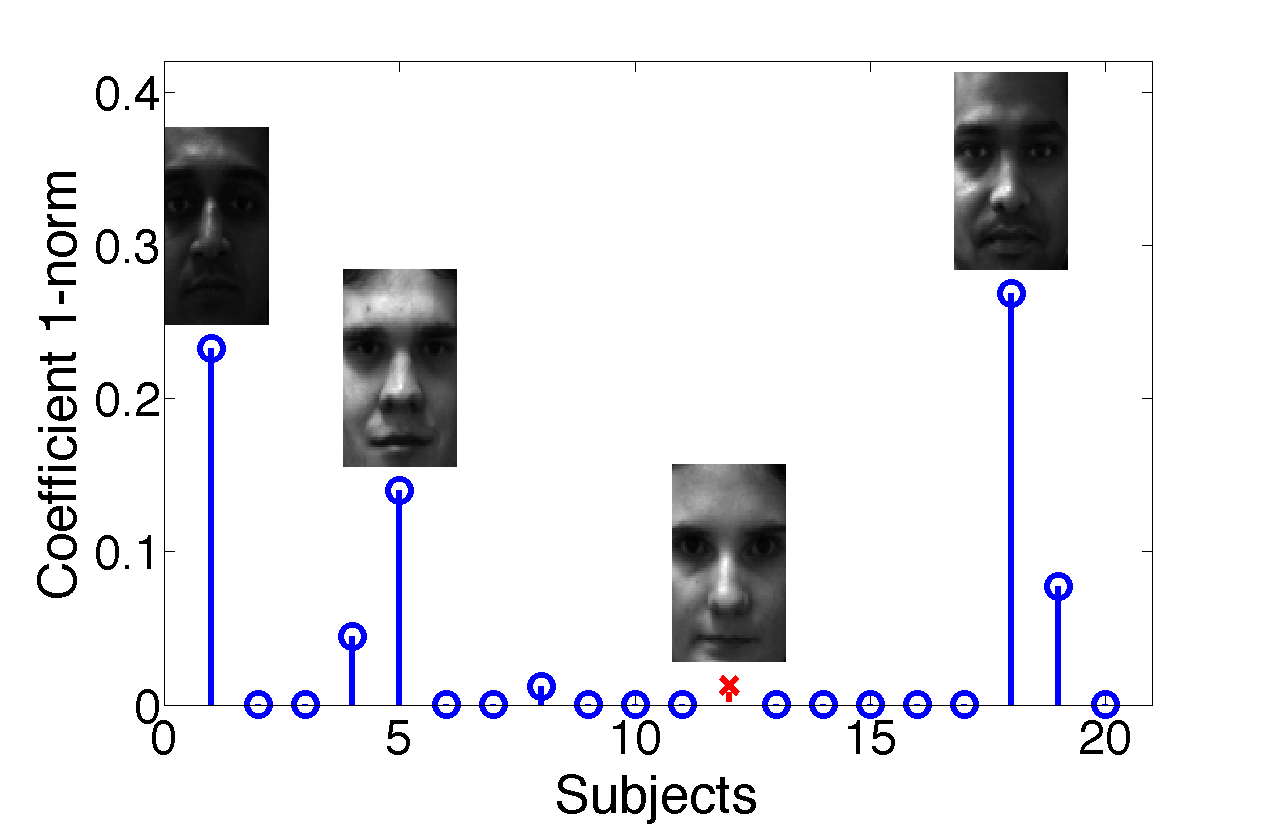
\includegraphics[height=1.2in]{figures_cvpr/promo/case2/sci_with_axis_face_case2.png} \\
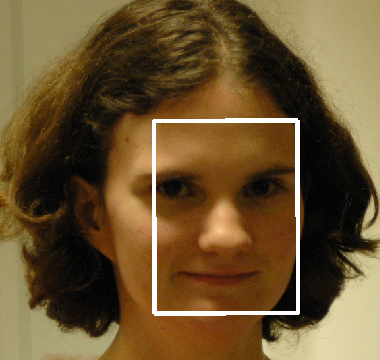
\includegraphics[height=1.2in]{figures_cvpr/promo/case3/alignment.png} & \hspace{3mm}
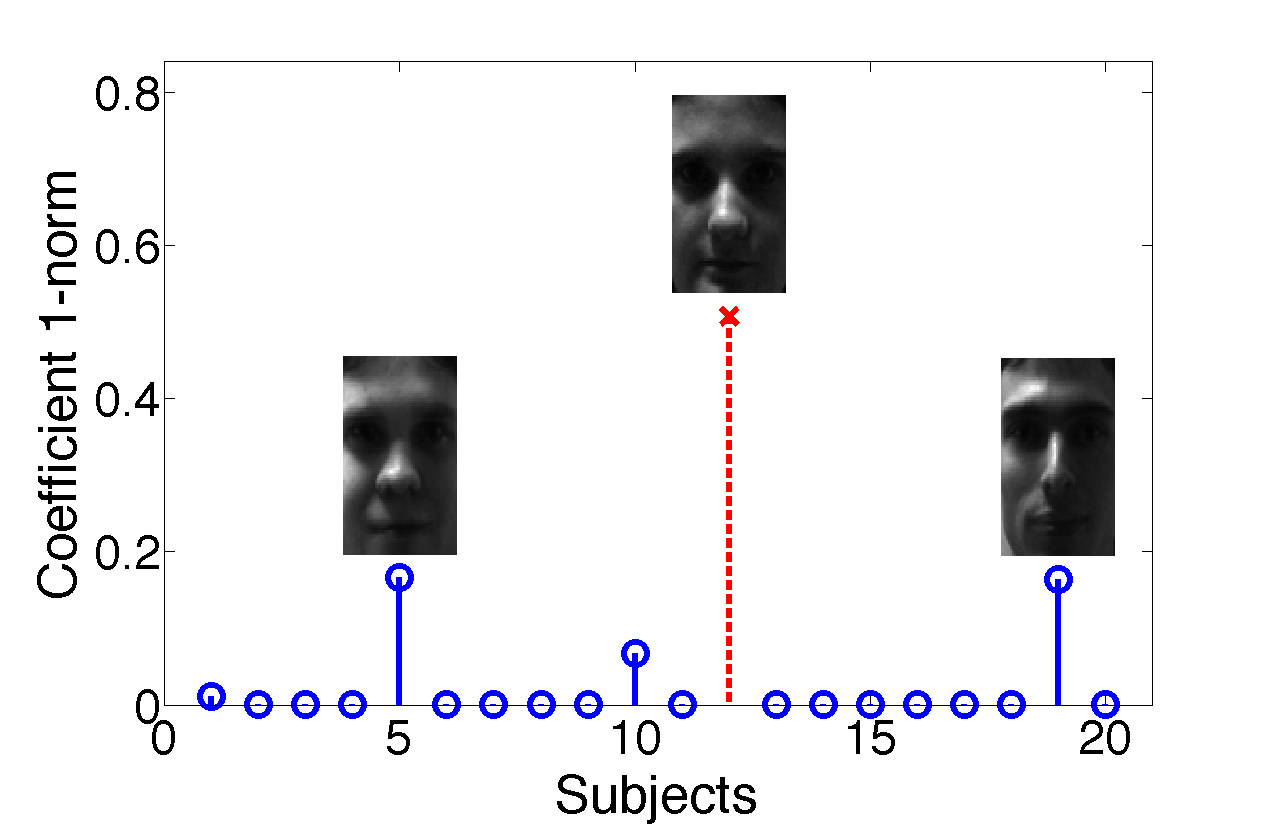
\includegraphics[height=1.2in]{figures_cvpr/promo/case3/sci_with_axis_face_case3.png}
\end{tabular}
\caption{{\bf Compound effect of registration and illumination}. The task is to identify the girl among 20 subjects, by computing the sparse representation of her input face with respect to the entire training set. The absolute sum of the coefficients associated with each subject is plotted on the right. We also show the faces reconstructed with each subject's training images weighted by the associated sparse coefficients. The red line (cross) corresponds to her true identity, subject 12. {\bf Top:} The input face is from Viola and Jones' face detector (the black box) and all 38 illuminations specified in Section \ref{sec:illumination} are used in the training.  {\bf Middle:} The input face is well-aligned (the white box) with the training by our algorithm specified in Section \ref{sec:registration} but only 24 frontal illuminations are used in the training for recognition (see Section \ref{sec:illumination}). {\bf Bottom:} Informative representation obtained by using both well-aligned input face and sufficient (all 38) illuminations in the training. \vspace{0mm}} 
\label{fig:promo}
\end{figure}

While that work achieves impressive results on public datasets taken under controlled laboratory conditions such as Extended Yale B \cite{Georghiades2001-PAMI}, it fails to address two critical aspects of real world face recognition: significant variations in both the {\em image domain} and in the {\em image value}. We illustrate this with an example in  Figure \ref{fig:promo}. The task is to identify the girl among 20 subjects. If the test face image, say obtained from an off-the-shelf face detector, has even a small amount of registration error against the training images (caused by mild pose, scale, or misalignment), the representation is no longer informative, even if sufficient illuminations are present in the training as shown in Figure \ref{fig:promo} top. In addition, in order to sufficiently interpolate the illumination of a typical indoor (or outdoor) environment, illuminations from behind the subject are also needed in the training. Otherwise, even for perfectly aligned test images, the representation will not necessarily be sparse or informative, as shown by the example in Figure \ref{fig:promo} middle. Unfortunately, most public face databases lack images with a significant component of rear (more than 90 degrees from frontal) illumination, either for training or testing.\vspace{0mm}

\paragraph{Contributions.} In this chapter, we show how the two {\em strongly coupled} issues of registration and illumination can be naturally addressed within the sparse representation framework. We show that face registration, a challenging nonlinear problem, can be solved by a series of linear programs that iteratively minimize the sparsity of the registration error. This leads to an efficient and effective alignment algorithm for face images that works for a large range of variation in translation, rotation, scale, and pose, even when the face is only partially visible due to eyeglasses, hats, closed eyes and open mouth, sensor saturation, etc.  We also propose a sufficient, if not the smallest, set of training illuminations that is capable of interpolating typical indoor and outdoor lighting, along with a practical hardware system for capturing them.  Finally, we demonstrate the effectiveness of the proposed new methods with a complete face recognition system that is {\em simple, stable, and scalable}. 
The proposed algorithm performs robust automatic recognition of subjects from loosely controlled images taken both indoors and outdoors, using labeled frontal views of the subjects' faces under the proposed illuminations for training and an off-the-shelf face detector\footnote{In this chapter, we use the OpenCV implementation of the Viola and Jones' face detector \cite{Viola2004-IJCV}.} to detect faces in images. \vspace{0mm}

\section{Handling Practical Registration Error}\label{sec:registration}\vspace{0mm}
As demonstrated in Figure \ref{fig:promo} top, the main limitation of the {\em sparse representation and classification} (SRC) algorithm of \cite{Wright2009-PAMI} is the assumption of pixel-accurate alignment between the test image and the training set. This leads to brittleness under pose and misalignment, making it inappropriate for deployment outside a laboratory setting. In this section, we show how this weakness can be rectified while still preserving the conceptual simplicity and good recognition performance of SRC. 

SRC assumes access to a database of multiple registered training images per subject, taken under varying illuminations. The images of subject $i$, stacked as vectors, form a matrix $A_i \in \Re^{m \times n_i}$. Taken together, all of the images form a large matrix $A = [ A_1 \mid A_2 \mid \dots \mid A_K ] \in \Re^{m \times n}$. As argued in \cite{Wright2009-PAMI}, a well-aligned test image $\y_0$ can be represented as a sparse linear combination $A \x_0$ of all of the images in the database,\footnote{We assume the illuminations in the training set are sufficient. We will address how to ensure illumination sufficiency in the next section.} plus a sparse error $\e_0$ due to occlusion. The sparse representation can be recovered by minimizing the sum or the 1-norm\footnote{The 1-norm of a vector $\x$ is the sum of absolute values of the entries.} of $\x$ and $\e$:\vspace{0mm}

\begin{equation}
\min \| \x \|_1 + \| \e\|_1 \quad \subj \quad \y_0 = A \x + \e.
\label{eqn:robust-l1}\vspace{0mm}
\end{equation}
Now suppose that $\y_0$ is subject to some pose or misalignment, so that instead of observing $\y_0$, we observe the warped image $\y = \y_0 \circ \tau^{-1}$, for some transformation $\tau \in T$ where $T$ is a finite-dimensional group of transformations acting on the image domain.  The transformed image $\y$ no longer has a sparse representation of the form $\y = A \x_0 + \e_0$, and naively applying the algorithm of \cite{Wright2009-PAMI} is no longer appropriate, as seen in Figure \ref{fig:promo} top. \vspace{0mm}

\paragraph{Batch and individual alignment.} Notice that if the true deformation $\tau^{-1}$ can be found, then we can apply its inverse $\tau$ to the test image and it again becomes possible to find a sparse representation of the resulting image, as $\y \circ \tau = A \x_0 + \e_0$.  This sparsity provides a strong cue for finding the correct deformation $\tau$: conceptually, one would like to seek a transformation $\tau$ that allows the sparsest representation, by solving\vspace{0mm}
\begin{equation} \label{eqn:L1-L1-conceptual}
\hat{\tau} = \arg\hspace{-2.5mm}\min_{\x,\e,\tau \in T} \| \x \|_1 + \| \e \|_1 \quad \subj \quad \y \circ \tau = A \x + \e. \vspace{0mm}
\end{equation}
For fixed $\tau$, this problem is jointly convex in $\x$ and $\e$. However, as a simultaneous optimization over the coefficients $\x$, error representation $\e$, and transformation $\tau$, it is a difficult, nonconvex optimization problem. One source of difficulty is the presence of multiple faces in the matrix $A$: \eqref{eqn:L1-L1-conceptual} has many local minima that correspond to aligning $\y$ to different subjects. In this sense, the misaligned recognition problem differs from the well-aligned version studied in \cite{Wright2009-PAMI}. For the well-aligned case, it is possible to directly solve for a global representation, with no concern for local minima. With possible misalignment, it is more appropriate to seek the best alignment of the test face with each subject $i$:\vspace{0mm}
\begin{equation} \label{eqn:per-subject-L1}
\hat \tau_i = \arg\hspace{-2.5mm}\min_{\x,\e,\tau_i \in T} \| \e \|_1 \quad \subj \quad \y \circ \tau_i = A_i \x + \e.\vspace{0mm}
\end{equation}
We no longer penalize $\| \x \|_1$, since $A_i$ consists of only images of subject $i$ and so $\x$ is no longer expected to be sparse.\vspace{0mm}

\paragraph{Alignment via iterative $\ell^1$-minimization.} While the problem \eqref{eqn:per-subject-L1} is still nonconvex, for cases of practical interest in face recognition, a good initial guess for the transformation is available, e.g., from the output of a face detector. We can refine this initialization to an estimate of the true transformation by repeatedly linearizing about  the current estimate of $\tau$, and seeking representations of the form:\vspace{0mm}
\begin{equation}
\y\circ \tau + J \Delta \tau = A_i \x + \e.\vspace{0mm}
\end{equation}
Here, $J = \frac{\partial}{\partial \tau} \y \circ \tau$ is the Jacobian of $\y \circ \tau$ with respect to the transformation parameters $\tau$, and $\Delta \tau$ is the step in $\tau$. The above equation is underdetermined if we allow the registration error $\e$ to be arbitrary. Near the correct alignment we expect the aligned testing image to differ from $A_i \x$ only for the minority of the pixels corrupted by occlusions. Thus, we seek a deformation step $\Delta \tau$ that best sparsifies of the registration error $\e$, in terms of its $\ell^1$-norm: \vspace{0mm}
\begin{equation}
\Delta\hat{\tau}_1 = \arg\hspace{-3.5mm}\min_{\x,\e,\Delta\tau \in T} \| \e \|_1 \quad \subj \quad \y + J \Delta \tau = A_i \x + \e.\vspace{0mm}
\label{eqn:L1-align}
\end{equation}
Notice that this is different from the popular choice that minimizes the 2-norm of the registration error:\vspace{0mm}
\begin{equation}
\Delta\hat{\tau}_2 = \arg\hspace{-3.5mm}\min_{\x,\e,\Delta\tau \in T} \| \e \|_2 \quad \subj \quad \y + J \Delta \tau = A_i \x + \e,\vspace{0mm}
\label{eqn:L2-align}
\end{equation}
which is also equivalent to finding the deformation step $\Delta  \tau$ by solving the least-square problem: $\min \|\y + J\Delta \tau - A_i \x \|_2$. Empirically, we find that if there is only small noise between $\y_0$ and $A_i\x$, both \eqref{eqn:L1-align} and $\eqref{eqn:L2-align}$ have similar performance.  However, if there are occlusions in $\y_0$, iterative $\ell^1$-minimization \eqref{eqn:L1-align} is significantly better than iterative $\ell^2$-minimization \eqref{eqn:L2-align}. Figure \ref{fig:L1-L2-align} shows an example.
\begin{figure}
\centering
\begin{tabular}{cccc}
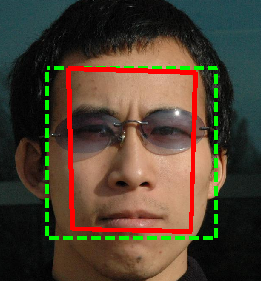
\includegraphics[height=1.2in]{figures_cvpr/L1_cropped} &

\includegraphics[height=1.2in]{figures_cvpr/y_warp_L1} &

\includegraphics[height=1.2in]{figures_cvpr/y_hat_L1} &

\includegraphics[height=1.2in]{figures_cvpr/e_L1} \\
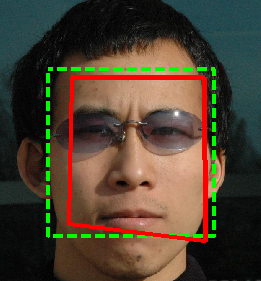
\includegraphics[height=1.2in]{figures_cvpr/L2_cropped} &

\includegraphics[height=1.2in]{figures_cvpr/y_warp_L2} &

\includegraphics[height=1.2in]{figures_cvpr/y_hat_L2} &

\includegraphics[height=1.2in]{figures_cvpr/e_L2} \\
(a) & (b) & (c) & (d)
\end{tabular}
\caption{{\bf Comparing alignment of a subject wearing sunglasses by 
$\ell^1$ and $\ell^2$ minimization.} 
{\bf Top:} alignment result of minimizing $\|\e\|_1$; {\bf Bottom:} 
result of minimizing $\|\e\|_2$. (a) {\em Green (dotted):} Initial face boundary
given by the face detector, {\em Red (solid):} Alignment result shown on the same
face; (b) warped testing image using the estimated transformation $\y_0$; 
(c) reconstructed face $A_i\x$ using the training; (d) image of error $\e$. \vspace{0mm}}\label{fig:L1-L2-align}
\vspace{0mm}\end{figure}

In addition to normalizing the training images (which is done once), it is important to normalize the warped testing image $\y \circ \tau$ as the algorithm runs.  Without normalization, the algorithm may fall into a degenerate global minimum corresponding to expanding a single black pixel in the test image.  Normalization is done by replacing the linearization of $\y \circ \tau$ with a linearization of the normalized version $\tilde \y(\tau) = \frac{\y \circ \tau}{\|\y \circ \tau\|_2}$.  The proposed alignment algorithm can be easily extended to work in a {\em multiscale} fashion, with benefits both in convergence behavior and computational cost.  The alignment algorithm is simply run to completion on progressively less down-sampled versions of the training and testing images, using the result of one level to initialize the next.  \vspace{0mm}

\paragraph{Robust recognition by sparse representation.}
Once the best transformation $\tau_i$ has been computed for each subject $i$, the training sets $A_i$ can be aligned to $\y$, and a global sparse representation problem of the form \eqref{eqn:robust-l1} can be solved to obtain a discriminative representation in terms of the entire training set. Moreover, the per-subject alignment residuals $\| \e \|_1$ can be used to prune unpromising candidates from the global optimization, leaving a much smaller and more efficiently solvable problem. The complete optimization procedure is summarized as Algorithm \ref{alg:deformable-src}. \vspace{0mm}
\begin{algorithm}[thb]
\begin{small}
\caption{\bf \small  (Deformable Sparse Recovery and Classification for Face Recognition).} \label{alg:deformable-src}
\begin{algorithmic}[1]
\STATE {\bf Input:} Frontal training images $A_1, A_2, \ldots, A_K \in \Re^{m\times n_i}$ for $K$ subjects,  a test image $\y\in\Re^m$ and a deformation group $T$ considered.
\STATE {\bf for} each subject $k$, 
\STATE \hspace{3mm} $\tau^{(0)} \leftarrow I$.
\STATE \hspace{3mm} {\bf do}
\STATE \hspace{6mm} $\tilde \y(\tau) \leftarrow \frac{\y \circ \tau}{\|\y \circ \tau\|_2}$; \;\;\; $J \leftarrow  \frac{\partial}{\partial \tau} \tilde\y(\tau)  \bigr|_{\tau^{(i)}} $;\vspace{0mm}
%\STATE \hspace{6mm} $(\hat \x, \hat \e, \Delta \tau) \leftarrow \left\{\begin{array}{l} \arg \min_{\x,\e,\Delta \tau} \| \e \|_1 \\  \subj \; \y + J \Delta \tau = A_k \x + \e \end{array}\right.$
\STATE \hspace{6mm} $ \Delta \tau =  \arg\min \; \| \e \|_1  \; \mathrm{s.t.} \; \tilde \y + J \Delta \tau = A_k \x + \e, \; \x \ge \0.$
\STATE \hspace{6mm} $\tau^{(i+1)} \leftarrow \tau^{(i)} + \Delta \tau$; 
\STATE \hspace{3mm} {\bf while} $\| \tau^{(i+1)} - \tau^{(i)} \| \ge \varepsilon$.
\STATE {\bf end}
\STATE Keep the top $S$ candidates $k_1, \ldots, k_S$ with the smallest residuals $\|\e\|_1$. 
\STATE Set $A \leftarrow \big[ A_{k_1} \circ \tau_{k_1}^{-1} \mid A_{k_2} \circ \tau_{k_2}^{-1} \mid \dots \mid A_{k_S} \circ \tau_{k_S}^{-1} \big]$. 
\STATE Solve the $\ell^1$-minimization problem: \vspace{0mm}
$$\hat{\x} = \arg \min_{\x, \e} \| \x \|_1 + \|\e\|_1 \;\; \text{subj} \;\; \y = A \x + \e, \;\x \ge 0.\vspace{0mm}$$
\STATE Compute residuals $r_i(\y) = \| {\y} - {A}_i \, \hat{\x}_i \|_2$ for $i = k_1, \dots, k_S$.
\STATE {\bf Output:} $\mbox{identity}(\y) = \arg\min_i r_i(\y)$.
\end{algorithmic}
\end{small}
\end{algorithm}\vspace{0mm}

The most important free parameter in Algorithm \ref{alg:deformable-src} is the class of deformations $T$. In our experiments, we typically use 2D similarity transformations, $T = \mathbb{SE}(2)\times \Re_+$, for compensating error incurred by face detector, or 2D projective transformations, $T = \mathbb{GL}(3)$, for handling some pose variation. The parameter $S$ decides how many top candidates get considered together to provide a sparse representation for the test image. If $S = 1$, the algorithm reduces to classification by registration error; but considering the test image might be an invalid subject, we typically choose $S = 10$. Since valid images have a sparse representation in terms of this larger set, we can reject invalid test images using the {\em sparsity concentration index} proposed in \cite{Wright2009-PAMI}. We have implemented a fast linear program for our algorithm in C. Running on a 2.8GHz Mac Pro, alignment takes 0.65 second per subject for our database. \vspace{0mm}


\paragraph{Simulations and experiments on region of attraction.} We now perform simulations and experiments demonstrating the effectiveness of the individual alignment procedure outlined in the previous section, and clarifying its operating range. We delay large-scale recognition experiments to Section \ref{sec:experiment}, after we have discussed the issue of illumination in the next section.\vspace{0mm}
\begin{enumerate}	
\item{\em 2D Deformation.}  We first verify the effectiveness of our alignment algorithm with images from the CMU Multi-PIE Database \cite{Gross2008-FGR}. We select 120 subjects in Session 2, use 11 illuminations per person from Session 2 for training, and test on one new illumination from Session 3.\footnote{The training are illuminations $\{0, 1,3,5,7,9,11,13,14,16,18\}$ of \cite{Gross2008-FGR}, and the testing is the illumination 10. } We manually select eye corners in both training and testing as the ground truth for registration. We down-sample the images to $80\times 60$ pixels\footnote{Unless otherwise stated, this will be the default resolution at which we prepare all our training and testing datasets and run all our experiments.} and the distance between the two outer eye corners are normalized to be 50 pixels for each person. We introduce artificial deformation to the testing image with a combination of translation or rotation. We consider a registration successful if the difference between the final registration error is within 1\% of the error by manual registration.  Figure \ref{fig:attraction} shows the percentage of successful registrations for the 120 subjects for each artificial deformation. The results suggest that our algorithm works extremely well with translation up to 20\% of the eye distance (or 10 pixels) in all directions and up to $30^\circ$ in-plane rotation. We have also tested our alignment algorithm with scale variation and it can handle up to 25\% change in scale.

We have gathered the statistics of the Viola and Jones' face detector on the Multi-PIE datasets. For 4,600 frontal images of 230 subjects under 20 different illuminations, using manual registration as the ground truth, the average misalignment error of the detected faces is about 6 pixels and the variation in scale is 17\%. This falls safely inside the range of attraction for our alignment algorithm.
\begin{figure}
\centering
\begin{tabular}{cc}
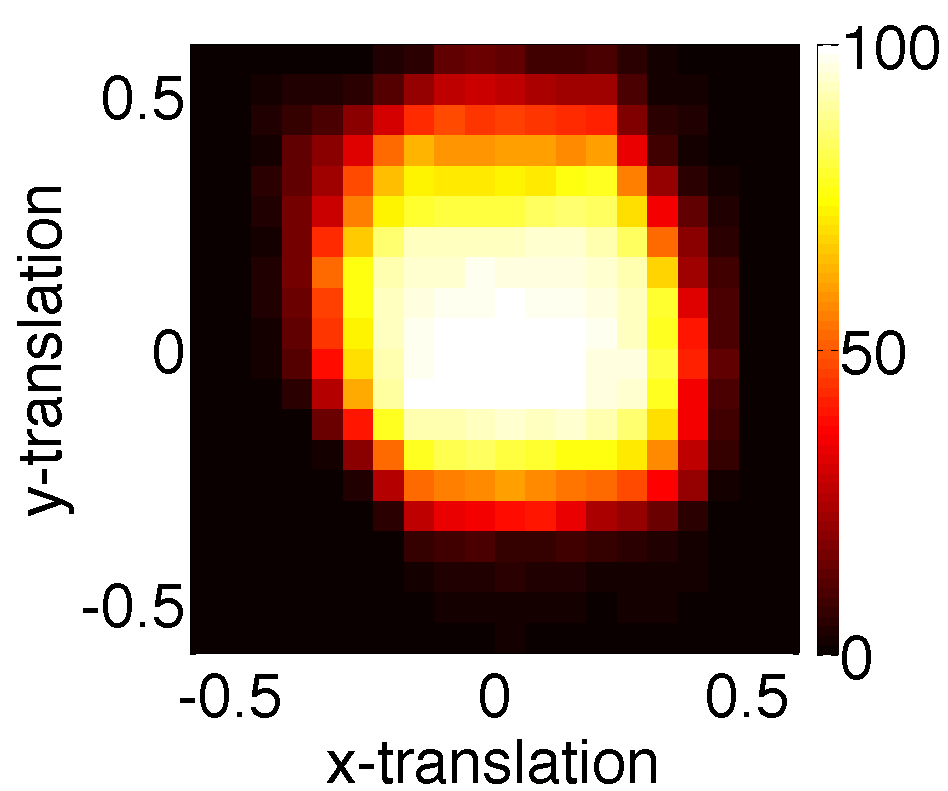
\includegraphics[height=1.8in]{figures_cvpr/translation_fig3.png} &
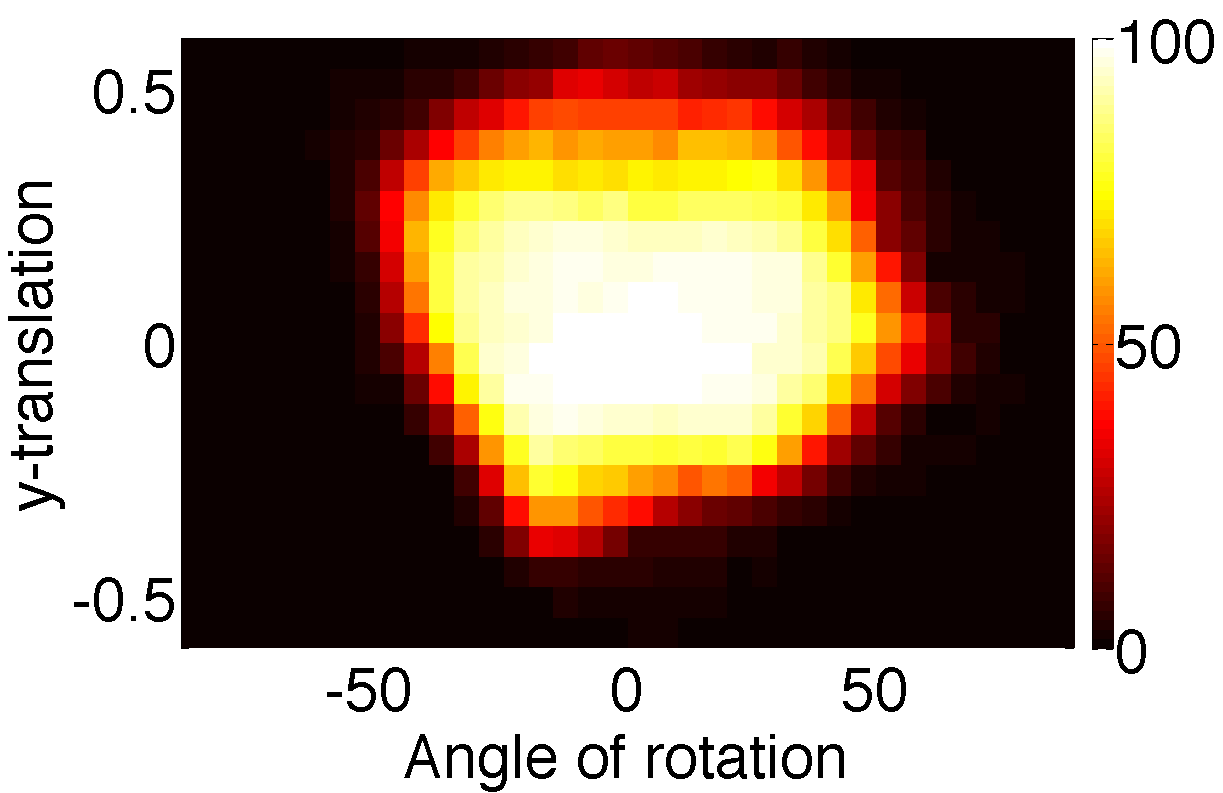
\includegraphics[height=1.9in]{figures_cvpr/translation_rotation_fig1.png}\\
(a)&(b)
\end{tabular}
\vspace{0mm}
\caption{{\bf Region of attraction.} Fraction of subjects for which the algorithm successfully aligns a synthetically perturbed test image.  The amount of translation is expressed as a fraction of the distance between the outer eye corners, and the amount of in-plane rotation in degrees. {\bf Left:} Simultaneous translation in $x$ and $y$ directions. More than $90\%$ of the subjects were correctly aligned for any combination of $x$ and $y$ translations, each upto $0.2$. {\bf Right:} Simultaneous translation in $y$ direction and in-plane rotation $\theta$. More than 90\% of the subjects were correctly aligned for any combination of $y$ translation upto $0.2$ and $\theta$ upto $25^\circ$.}
\label{fig:attraction}
\end{figure}

\vspace{0mm}
\item{\em 3D Pose Variation.} As densely sampled pose and illumination face images are not available in any of the public databases, including Multi-PIE, we have collected our own dataset using our own system (to be introduced in the next section.) We use frontal face images of a subject under the 38 illuminations proposed in the next section as training. For testing, we collect the image of the subject under a typical indoor lighting condition at pose ranging from $-90^\circ$ to $+90^\circ$ with step size 5.625$^\circ$, a total of 33 poses. We use Viola and Jones' face detector to initialize our alignment algorithm. 
%whenever it succeeds. For extreme poses where the detector fails (usually for poses $> 45^\circ$), we use manual initialization by putting a reasonable square window around the face. 
Figure \ref{fig:pose-alignment} shows the typical alignment results of our algorithm, working surprisingly well with poses up to $\pm 45^\circ$. \vspace{0mm}
\begin{figure}
\centering
\begin{tabular}{ccccc}

\includegraphics[height=1in]{figures_cvpr/5} &
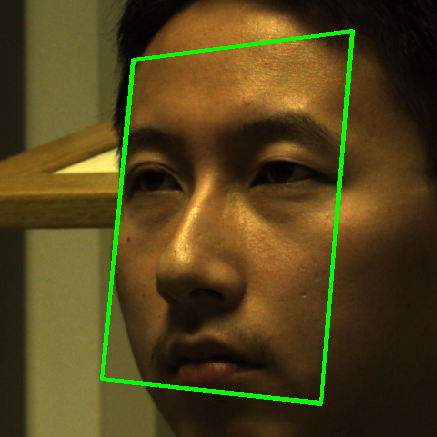
\includegraphics[height=1in]{figures_cvpr/7} &
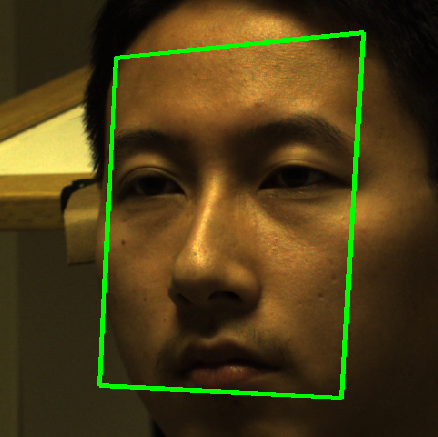
\includegraphics[height=1in]{figures_cvpr/09} &
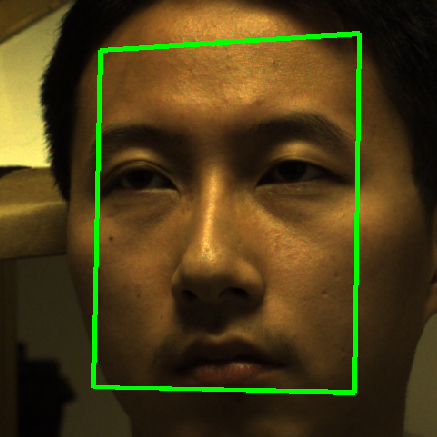
\includegraphics[height=1in]{figures_cvpr/11} &
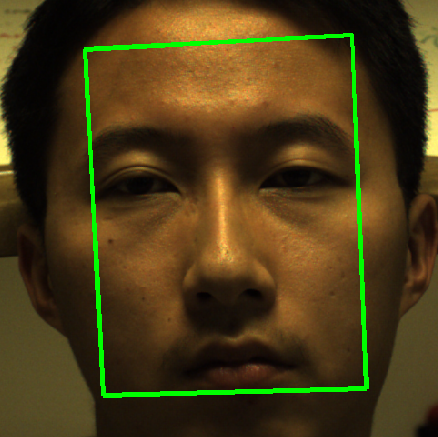
\includegraphics[height=1in]{figures_cvpr/13} \\
(a) & (b) & (c) & (d) & (e)\vspace{3mm}\\
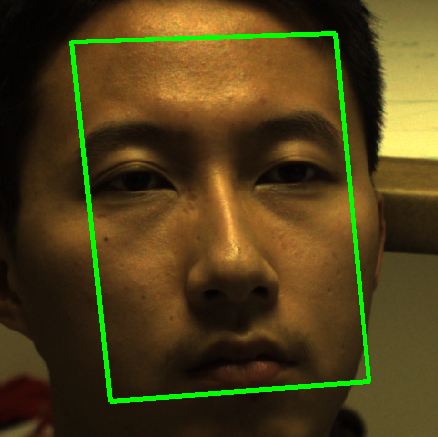
\includegraphics[height=1in]{figures_cvpr/15} &

\includegraphics[height=1in]{figures_cvpr/17} &
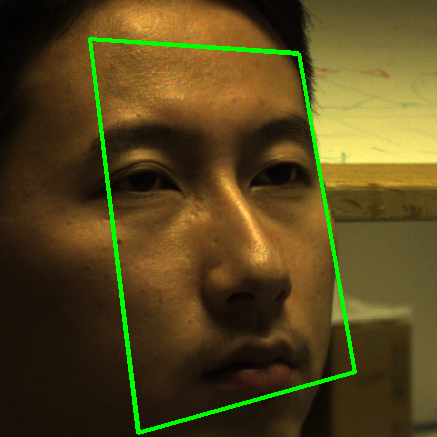
\includegraphics[height=1in]{figures_cvpr/19} &
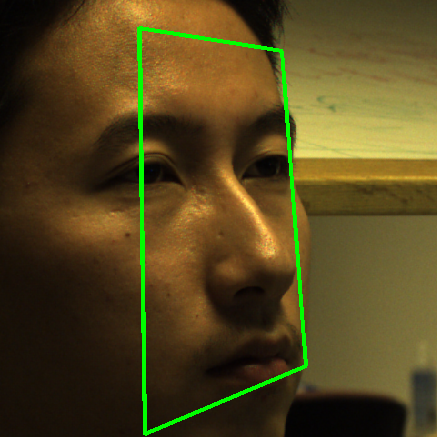
\includegraphics[height=1in]{figures_cvpr/21} &

\includegraphics[height=1in]{figures_cvpr/3} \\
(f) & (g) & (h) & (i) & (j)
\end{tabular}
\caption{{\bf Aligning different poses to frontal training images.} {\bf (a) to (i):}  good alignment for pose from $-45^{\circ}$
to $+45^{\circ}$. {\bf (j):} a case when the algorithm fails for an extreme pose ($>45^{\circ}$).\vspace{0mm}
}\label{fig:pose-alignment}
\end{figure}
\end{enumerate}

\paragraph{Relationship to existing work.} 
Our modification to SRC roots solidly in the tradition of adding deformation-robustness to face recognition algorithms \cite{Cootes2001-PAMI,Gross2006-PAMI,Wiskott1997-PAMI}. However, the only previous work to investigate face alignment in the context of sparse signal representation and SRC is the work of \cite{Huang2008-CVPR}. They consider the case where the training images themselves are misaligned and allow one deformation per training image. They linearize the training rather than the test, which is computationally more costly as it effectively triples the size of the training set. In addition, as they align the test image to all subjects simultaneously, it potentially is more prone to local minima when the number of subjects increases, as we will see in the following experimental comparisons. \vspace{0mm}
\begin{enumerate}
\item {\em Extended Yale B.} In this experiment, we have used the exact experimental settings in \cite{Huang2008-CVPR}. 
20 subjects are selected and each has 32 frontal images (selected at random) as training and another 32 for testing. An artificial translation
of 10 pixels (in both $x$ and $y$ directions) is introduced to the test. For our algorithm we down-sample all the images
to $88\times 80$ for memory reasons, whereas the work of \cite{Huang2008-CVPR} uses random projections. Our algorithm achieves the recognition rate 88.59\% which is on par with the result reported in \cite{Huang2008-CVPR}.
However, this special setting is disadvantageous to our algorithm: The use of cropped test images introduces boundary effects, and the presence of very extreme illuminations makes enforcing nonnegativity of $\x$ (as in Algorithm 1 less appropriate. We further discuss the justification for nonnegativity in the next section.\vspace{0mm}
\item {\em CMU Multi-PIE.} In this experiment, we choose 160 subjects from the CMU Multi-PIE, 11 training images from Session 2
and 1 test image from Session 3 per person. The setting is exactly the same as the previous experiment on 2D deformation, 
except that we have more subjects. We again 
work with downsampled images of size $80\times 60$. An artificial translation of 5 
pixels (in both $x$ and $y$ directions) was induced in the test image. The algorithm of \cite{Huang2008-CVPR} achieves
a recognition rate of 73.75\%,\footnote{That algorithm has two free parameters - $l$ and $d$. For this experiment we chose 
$l = 1$ and $d = 514$ (higher values may get a better recognition rate at the expense of higher running time).
} while ours does 90.625\%. \end{enumerate}\vspace{0mm}
				
\section{Handling Practical Illumination Variation}\label{sec:illumination}\vspace{0mm}
In the above section, we have made the assumption that the test image, although taken under some arbitrary illumination, can be linearly interpolated by a finite number of training illuminations.  Under what conditions is this a reasonable assumption to make?  What can we say from first principles about how the training images should be chosen?  

\paragraph{The illumination model}
First, let us assume that the illumination if the subject's face is distant.  This model will be a good approximation as long as distance to the nearest light source is much larger than the person's face.  If we further assume that the object is convex so that there is no self-shadowing, the illumination incident on a surface patch will depend only on its orientation, and not on its position.  Furthermore, if the object is lambertian, the intensity of the image of a given patch of object will not depend on its position either.  Since each pixel in the image corresponds to some patch on the object, the vector of image intensities is a linear function of the radiance of the corresponding portions of the object.  Consider the vector space of all illuminations of the object.  These are just positive functions (or more generally, distributions) defined on the sphere, where each point on the sphere corresponds to a direction of incoming light.  Consider the vector space formed by the light exiting the object.  This too is a positive function defined on the sphere, where now each point on the sphere corresponds to the normal of a patch on the object (or any other patch with the same normal).  Under the Lambertian assumption, the radiance of a patch depends on the cosine of the incident angle of incoming light, and is integrated over the half-sphere of illumination that the patch can "see".
Thus, the surface of the object acts on the sphere in a manner very similar to a half-cosine approximation to a low-pass filter for a one-dimensional signal.  Thus the energy leaving the object is disproportionately concentrated in the subspace corresponding to low spatial frequencies.  Since the image is a linear function of this, the space of images of an object will also tend to fall on (the positive portion of) a subspace.   In \cite{Basri2003-PAMI}, Basri showed using spherical harmonic basis functions that nine basis illuminations (corresponding to the lowest frequency spherical harmonics) result in training images that do a good job of linearly interpolating all other training images.  It should be noted, however, that these basis illuminations are not strictly positive, and thus neither are the training images they generate (when rendered on a computer that can handle negative illumination).  \footnote{Note that while the spherical harmonic basis functions have regions where they are negative, this does no necessary preclude this theoretical result from being put to use in practice.  If the geometry of the training illumination system were well calibrated, it would be possible to generate approximations of the positive and (rectified) negative components of the basis illuminations separately, taking the difference of the resulting two images, and storing it using a signed datatype.  Combinations of these images may not be positive, but they may still be good enough to be useful}.

Although a human face is neither perfectly Lambertian nor convex, it has been observed in various empirical studies that one can often get away using a similar number of frontal illuminations to interpolate a wide range of new frontal illuminations that taken under the same laboratory conditions \cite{Georghiades2001-PAMI}. This is the case for many public face datasets, including AR, ORL, PIE, and Multi-PIE.  Unfortunately, we have found that in practice, a training database consisting purely of frontal illuminations is not sufficient to linearly interpolate images of a faces taken under typical indoor or outdoor conditions (see the experiment conducted in Section \ref{sec:own-data}). As illustrated by the example in Figure \ref{fig:promo}, an insufficient number of training illuminations can result in recognition failure. 
To ensure our algorithm works in practice, we need to find a set of training illuminations that are indeed {\em sufficient} to linearly interpolate a wide variety of practical indoor and outdoor illuminations.\vspace{0mm}

\paragraph{Capturing a sufficient set of training illuminations.}   To this end, we have designed a system that can illuminate the subject from all directions above horizontal, while acquiring the subject's frontal images. A sketch of the system is shown in Figure \ref{fig:system}: The illumination system consists of four projectors that display various bright patterns onto the three white walls in the corner of a dark room.  The light reflects off of the walls and illuminates the user's head indirectly.  After taking the frontal illuminations we rotate the chair by 180 degrees and take pictures from the opposite direction.  Having two cameras speeds the process since only the chair needs to be moved in between frontal and rear illuminations.  
Our projector-based system has several advantages over flash-based illumination systems:\vspace{0mm}
\begin{itemize}
\item The illuminations can be defined in software.\vspace{0mm}
\item It is easy to capture many different illuminations.\vspace{0mm}
\item There is no need to mount cameras on walls or construct a large dome.\vspace{0mm}
\item No custom hardware is needed for a basic system.\vspace{0mm}
\end{itemize}
\begin{figure}
\centerline{\hspace{-0.1in}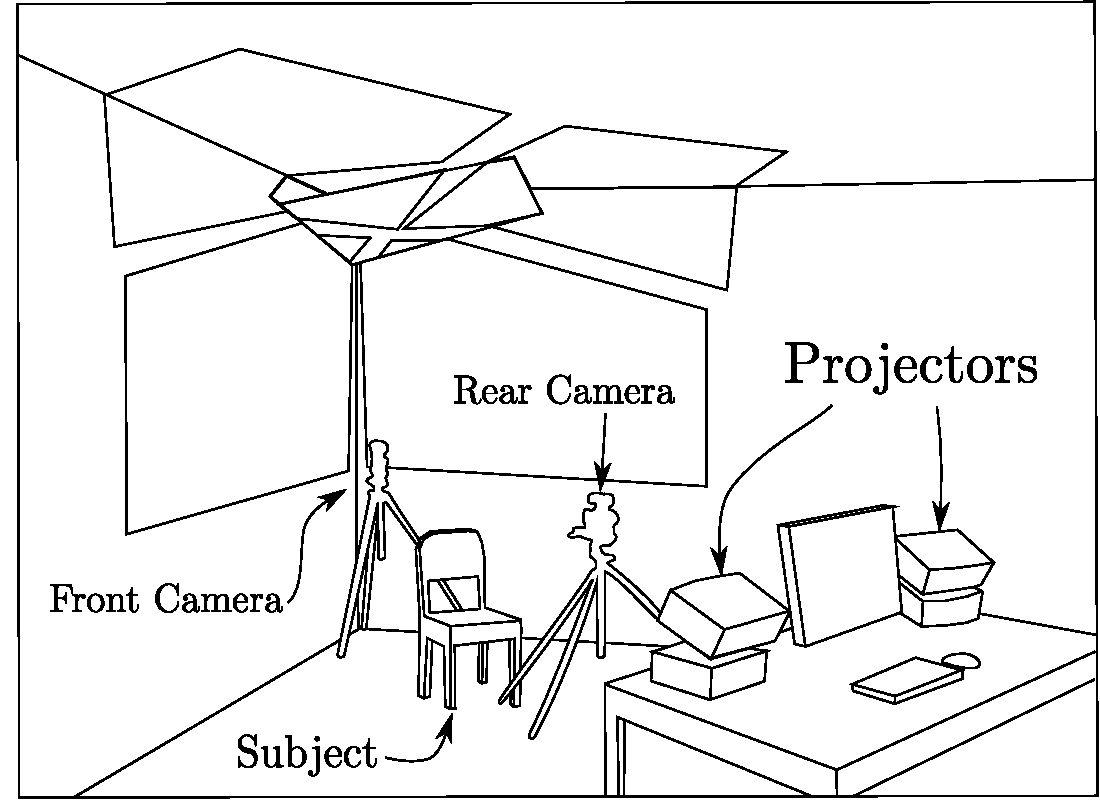
\includegraphics[height=3in]{figures_cvpr/camera_rig.pdf}}
\caption{{\bf Training acquisition system:} Four projectors and two cameras controlled by one computer.\vspace{0mm}}
\label{fig:system}
\end{figure}
With our projector system, our choice of illuminations is constrained only by the need to achieve a good SNR\footnote{Since illuminations with more pixels illuminated will have a better SNR (provided they don't saturate), there is an engineering tradeoff between the SNR and the number of training images we can acquire.}
avoid saturation, and achieve a reasonably short acquisition time.  Two simplifying assumptions that we make is that every pixel is either turned full on or off in every illumination, and that no pixels are shared by illuminations.  Assuming that the pixels are all the way on or all the way off allows us to control the amount of illumination directly with the number of pixels we illuminate, eliminating any influence from gamma curve of the projector. \footnote{Caution; DLP projectors may have very wacky response curves depending on the mode they are in.  Note that controlling the intensity between illuminations is only needed to prevent saturation or low SNR; our algorithm depends on the linearity between the illuminations and the images, not on the relative intensities of the illuminations.} The choice of orthogonal (no pixels in common) illuminations is important; any other non-negative basis illuminations formed from a linear combination of our basis vectors will span a cone of lower volume, and thus the resulting training images might not be able to represent as wide a variety of testing images. 

We ran two experiments to guide our choice of illuminations for our large-scale experiments:\vspace{0mm}  
\begin{itemize}
\item {\em Coverage Experiment.} In the first experiment we attempt to determine what coverage of the sphere is required to achieve good interpolation for test images.  The subject was illuminated by 100 (50 front, 50 back) illuminations arranged in concentric rings centered at the front camera.  Subsets of the training images were chosen, starting at the front camera and adding a ring at a time.  Each time a ring was added to the training illumination set, the average $\ell^1$ registration error (residual) for a set of test images taken under sunlight was computed and plotted in Figure \ref{fig:illumination-patterns} (a).  The more rings of training illuminations are added, the lower the representation error becomes, with diminishing returns.\vspace{0mm}
\item {\em Granularity Experiment.} In the second experiment we attempt to determine how finely divided the illumination sphere should be.  At the first granularity level, the projectors  illuminate the covered area uniformly.  At each subsequent granularity level each illuminated cell is divided in two along its longer side but intensity doubled.  For each granularity level the average $\ell^1$ registration error is computed as in the coverage experiment and shown in Figure \ref{fig:illumination-sufficiency} (b).  Again, diminishing returns are observed as more illuminations are added.\vspace{0mm}  
\end{itemize}
\begin{figure}
\centering
\begin{tabular}{cc}
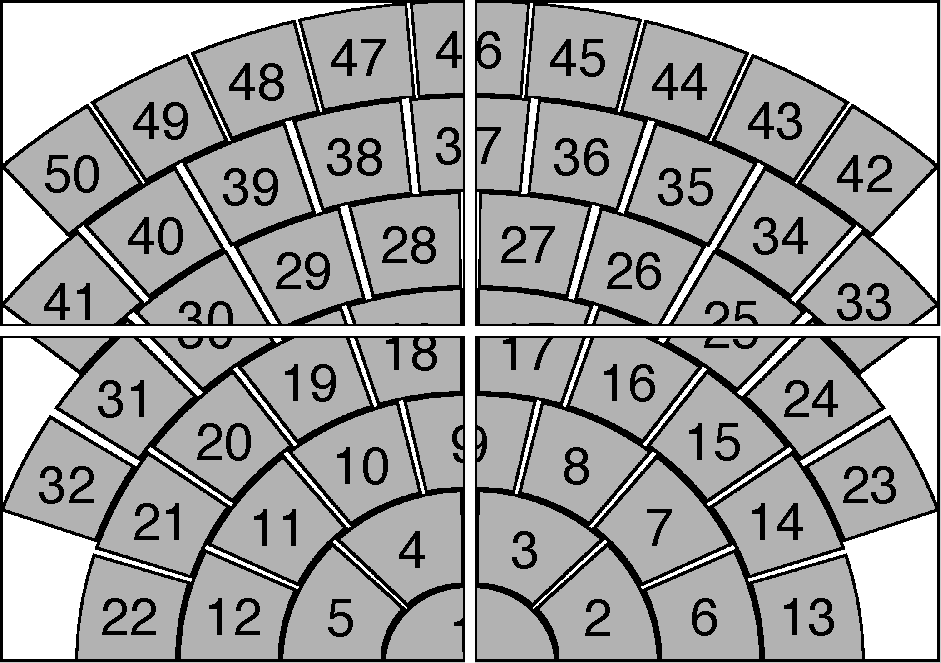
\includegraphics[height=2in]{figures_cvpr/coverage_experiment_asplode.png} &
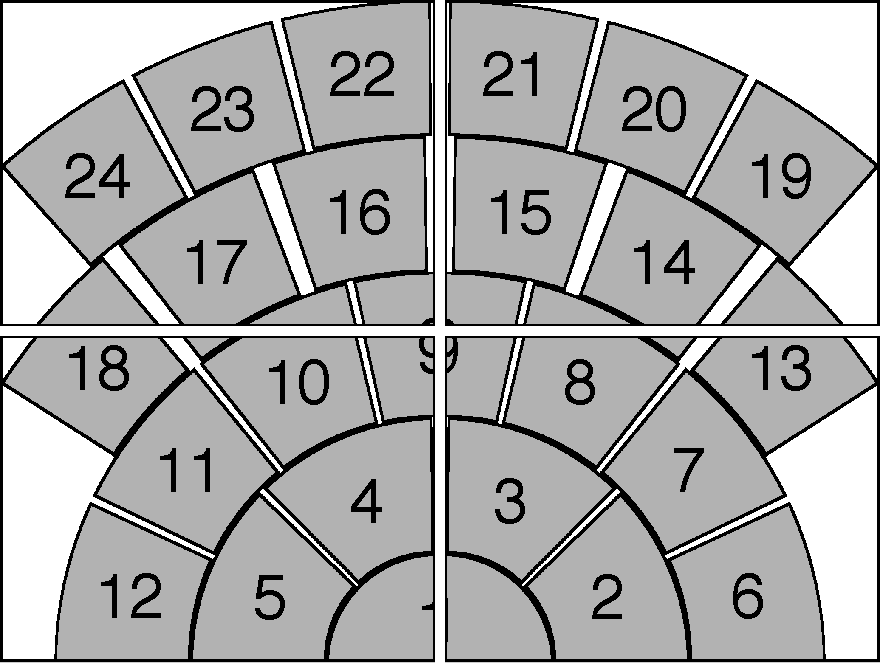
\includegraphics[height=2in]{figures_cvpr/final_cvpr_illuminations_asplode.png} \\
(a) Coverage Experiment & (b) Chosen Illumination Patterns
\end{tabular}\vspace{2mm}
\caption{{\bf Illumination patterns.}   The cells are illuminated in sequence.  For rear illuminations the sequence is reversed.  In the chosen pattern's rear illumination, the cells 1-5 and 7-11 are omitted for a total of 38 illuminations. The four rectangular regions correspond to the four projectors.\vspace{0mm}}
\label{fig:illumination-patterns}
\end{figure}
\begin{figure}
\centering
\begin{tabular}{cc}
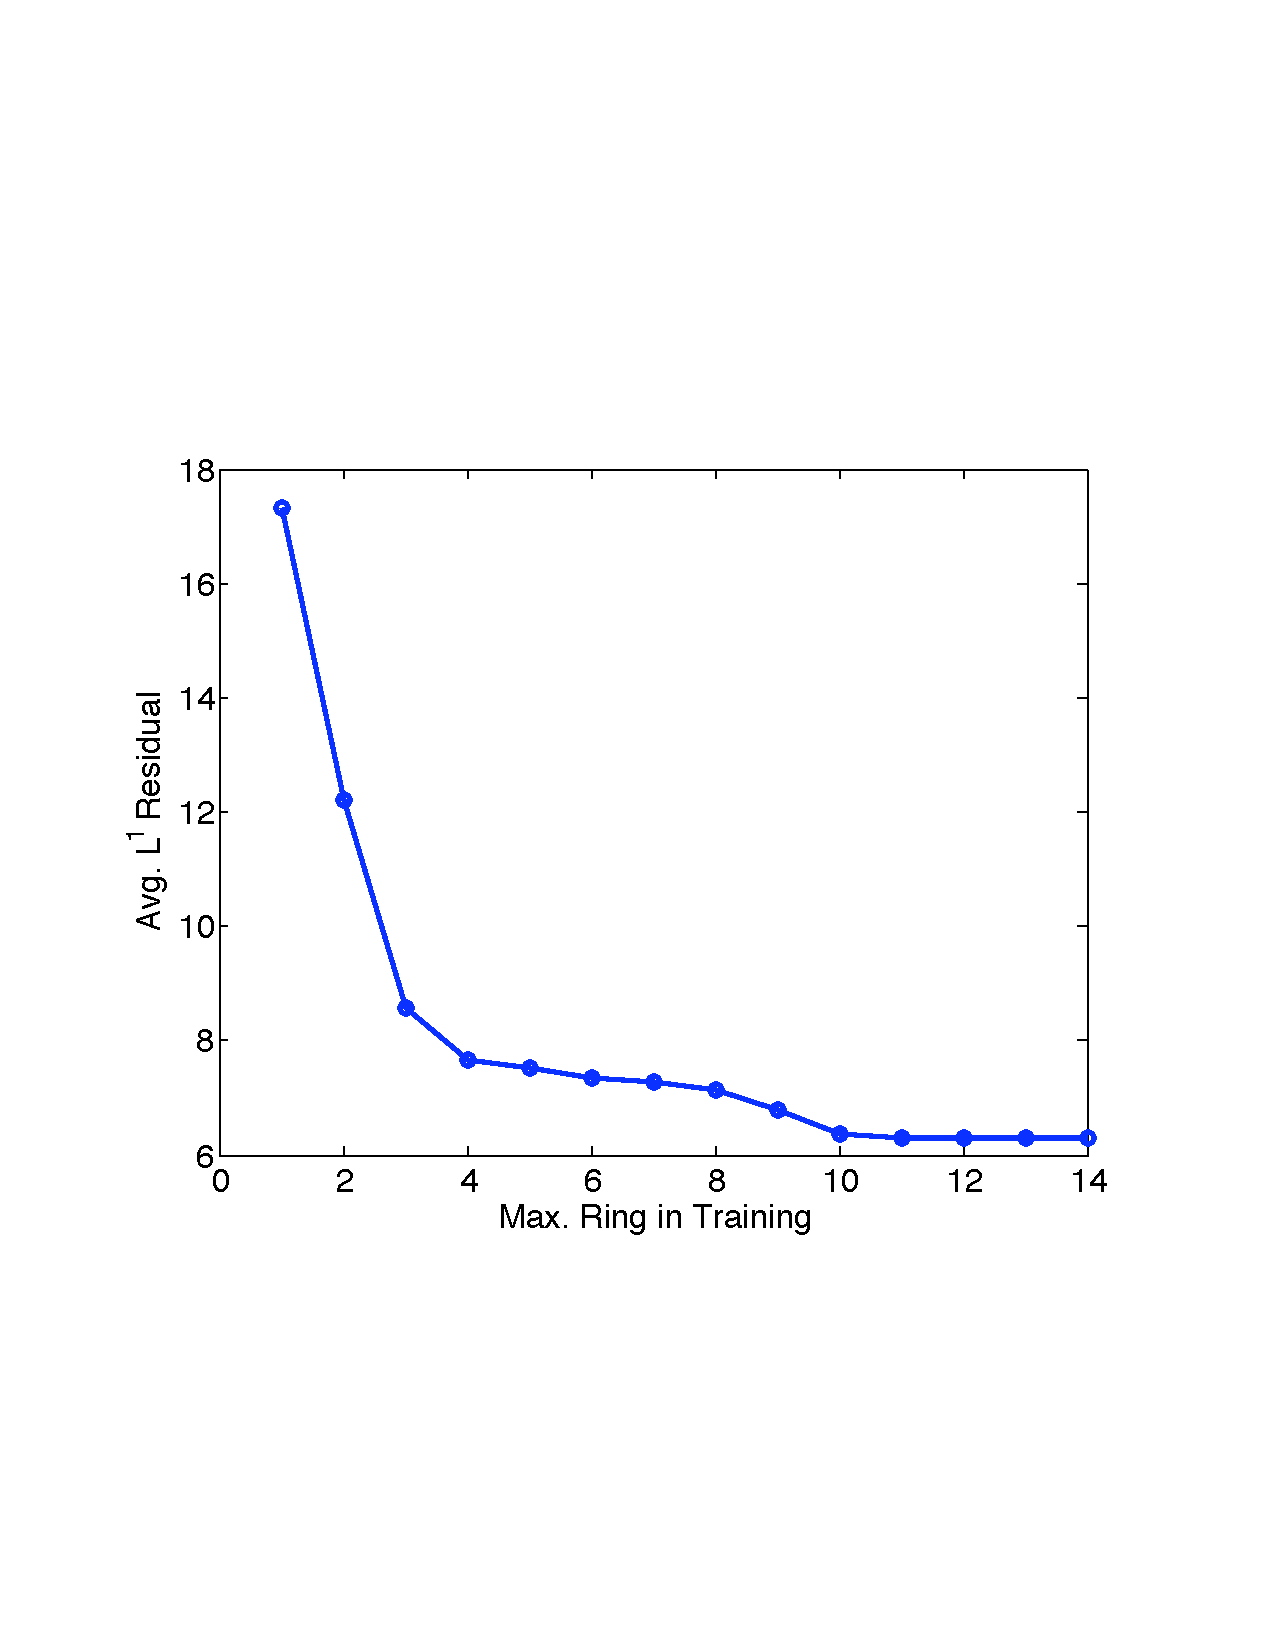
\includegraphics[height=1.5in]{figures_cvpr/illum_results/coverage_sunset.pdf} &
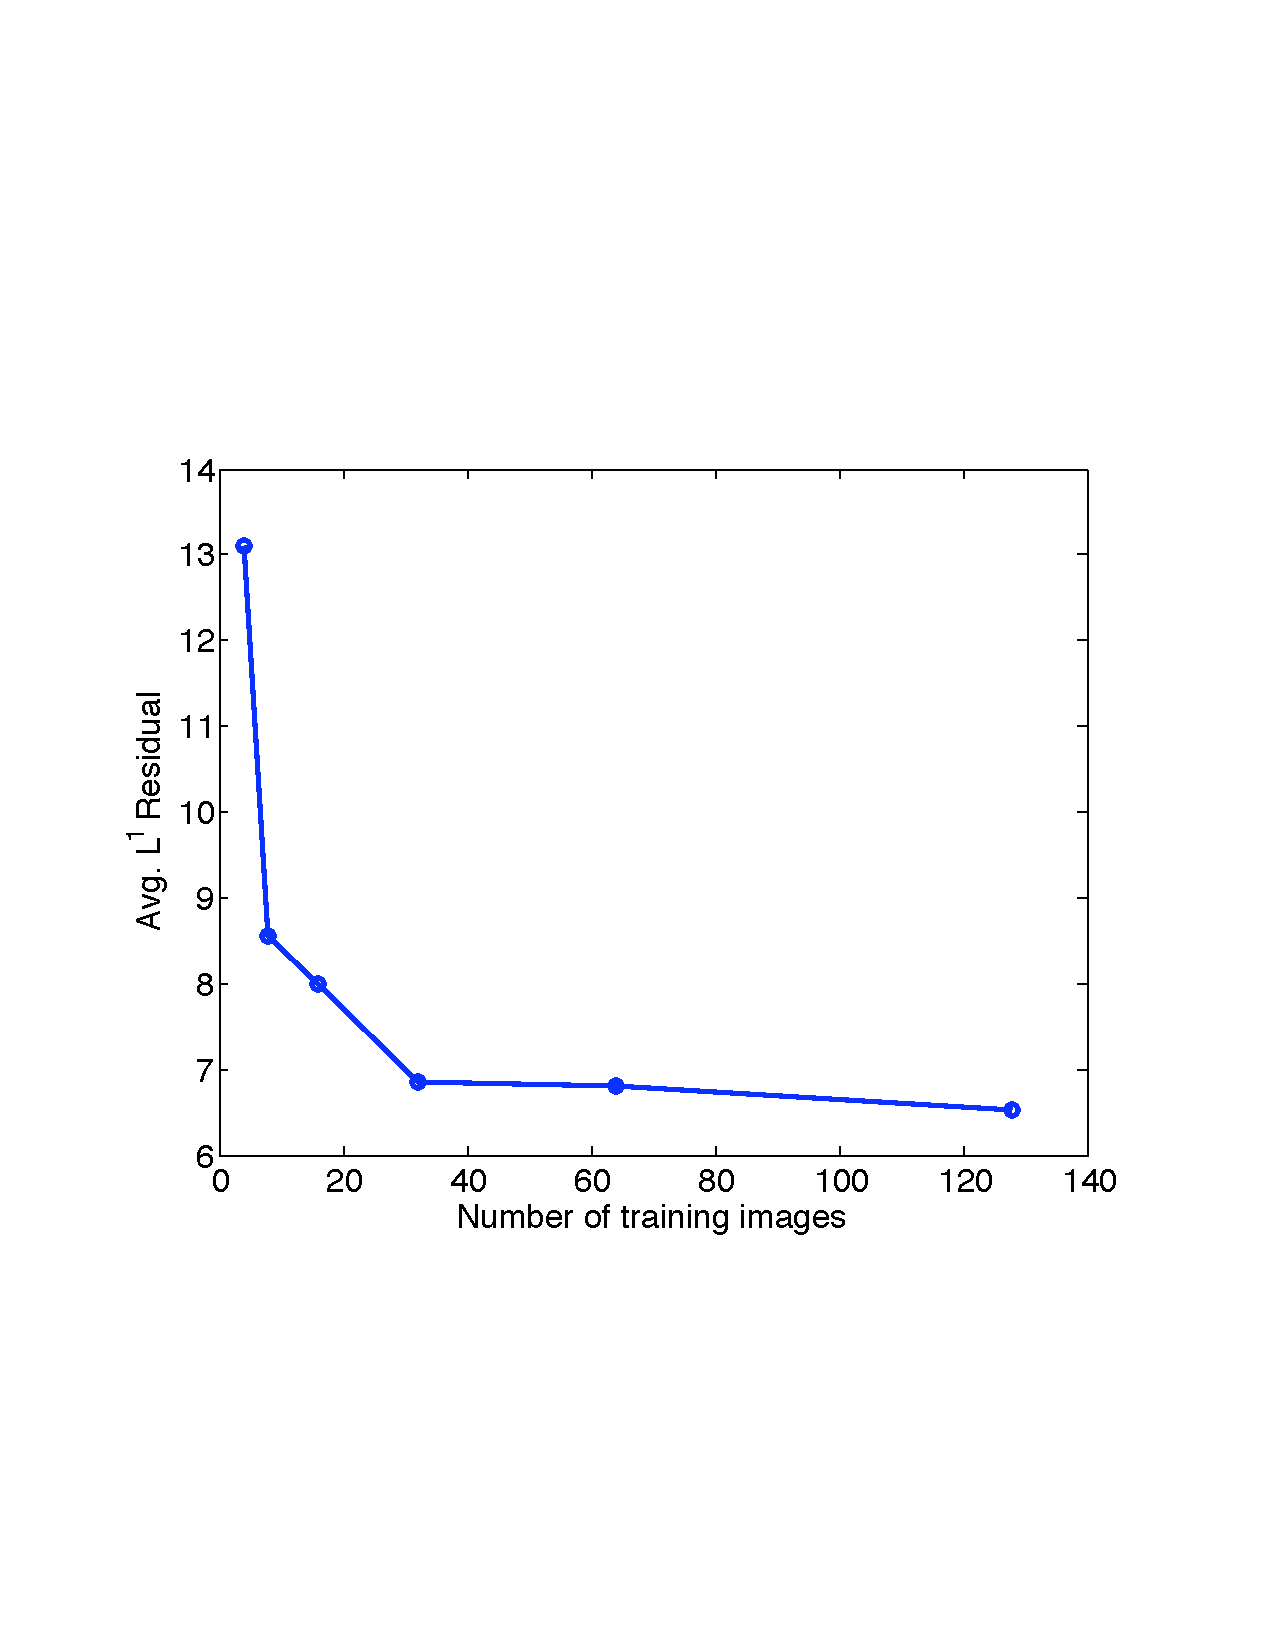
\includegraphics[height=1.5in]{figures_cvpr/illum_results/granularity_sunset.pdf} \\
(a) Coverage & (b) Granularity
\end{tabular}\vspace{2mm}
\caption{{\bf Study of sufficient illuminations.} The average $\ell^1$ registration residual versus different illumination training sets. \vspace{0mm}}
\label{fig:illumination-sufficiency}
\end{figure}

\vspace{0mm}\paragraph{Chosen illumination patterns.} In the plot for the coverage experiment, Figure \ref{fig:illumination-sufficiency} (a), we clearly see two plateau regions: one is after 4 rings and one is after 10 rings. The first four rings represent the typical frontal illuminations, which are present in most public face datasets; however, we see that the residual stabilizes after 10 rings which include some illuminations from the back of the subject. This suggests that although the frontal illuminations can span majority of illumination on the face, some illuminations from the back are needed in the training to emulate the effect of ambient illumination from all directions. In the plot for the granularity experiment, Figure \ref{fig:illumination-sufficiency} (b), we observe that the residual reaches a plateau after four divisions, corresponding to a total of 32 illuminations. Based on the results from both experiments, we decide to partition the area covered by the first 10 rings into a total of 38 cells, whose layout is explained in Figure \ref{fig:illumination-patterns} (b). For our large-scale experiments, we have collected those illuminations for all our subjects.\footnote{It is very likely that with more careful experiments, we can further reduce the number of illuminations needed. Especially some of the frontal illuminations might be redundant. But we keep those in our training anyway as the additional images do not add too much cost to our alignment and recognition algorithm.} 

See below for the 38 images for one subject:
\begin{figure}[h]
\centering
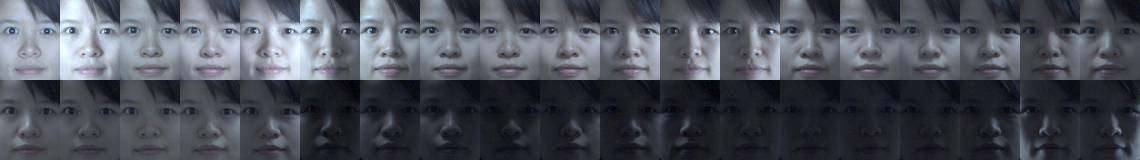
\includegraphics[width=6.3in]{figures_cvpr/training.png}
\end{figure}
\vspace{0mm}

\paragraph{Should Positivity in the Representation Coefficients be Enforced?}
One critical issue in linear illumination models is whether to enforce nonnegativity in the coefficients $\x$, i.e. whether to model illumination using a cone or a subspace.   Some authors, i.e. \cite{Basri2003-PAMI}, have chosen to allow negative components in the coefficient vector $\x$ when representing one image as a sum of other images, and only enforce that the linear combination $A\x$ be positive everywhere.  Unfortunately, for non-convex objects such as faces, enforcing non-negativity of the representation is not sufficient to guarantee that the resulting image of the object is physical.  For example, consider a Lambertian planar object with a cylindrical hole drilled in it that is aligned with the optical axis of an orthographic camera.  Consider two images: one under illumination from a distant point source aligned with the hole, and one off of the hole axis.  Positively weighting the on-axis image and negatively weighting the on-axis image can result in an image where the bottom of the hole is more strongly illuminated than the surrounding plane.  The image is positive, but it is clearly non-physical.  It is worth emphasizing that this phenomenon is a result of some points on an object seeing a restricted subset of the illumination sphere (a violation of convexity),  and not a result of the directionality of the light chosen in the thought experiment.  While the number of coefficients that actually end up negative after optimization is usually very small, we have observed pathological cases where the shadows next to the user's nose in the reconstructed image invert in value.  

Instead of using a smaller set of training images, allowing the coefficients to go negative to try to represent more test illuminations, and risking over-fitting, we decided to enforce non-negativity of the coefficients.  Nonnegative combinations of images are guaranteed to correspond to physically plausible images.  all physical illuminations unless the training images actually span the boundary of the illumination cone. 
Because we have a flexible acquisition system, we can directly generate a set of illuminations that span most of the illumination cone, without resorting to negative coefficients and risking overfitting.  Thus, in Algorithm 1, we have enforced that the coefficients $\x$ be non-negative.

%One of the main factors that complicates face recognition, and computer vision in general, is that two images of the same person's face can be very different, even if the pose is carefully controlled and all points on the person's face are visible in both images.  The most safe, reliable, and general assumption that can be made about the imaging process is that it is linear with respect to the intensity of different light sources.  The set of images of a given object is therefore a cone in the non-negative orthant of the pixel basis.  All recognition algorithms that rely on vision for training rely on images sampled from this cone.  

\paragraph{Compensating for Gamma Compression.}
Any algorithm based on representing a testing image as a weighted sum of training images must make sure that the image intensity has been coded linearly with image intensity.  Unfortunately, this cannot be taken for granted.  While most modern machine vision cameras capture linearly in intensity, older analog video cameras often used NTSC defined gamma compression, while most modern digital consumer and SLR cameras record in sRGB defined gamma compression.  Since not all algorithms depend on a linear image coding, there are several public face recognition databases that do not specify the gamma compression of their images.  Unfortunately, it is very easy to forget to deal with gamma correction properly; many algorithms (including ours) will not fail catastrophically if gamma is not handled correctly, but will likely not perform as well.  It is notable that the popular OpenCV library API does not contain built-in support for gamma decompression, yet contains many functions that perform linear operations on images.  Worse, several common image file formats fail to specify the gamma encoding of the data they contain.  The performance of the algorithm presented in this chapter benefits greatly from proper gamma decompression of the training and testing images.  

\section{Overall System Evaluation}\label{sec:experiment}\vspace{0mm}
In this section, to verify the performance of our algorithm and system, we conduct comprehensive experiments on large-scale face databases. We first test on the largest public face database available that is suitable for testing our algorithm, the CMU Multi-PIE. The goal is to show that our algorithm can indeed be used to achieve good performance on such a dataset with test images obtained from an off-the-shelf face detector, even though we can only use a small number of, not necessarily sufficient, training illuminations. We then test our algorithm on a face dataset that is collected by our own system. The goal is to show that with a sufficient set of training illuminations for each subject, our algorithm indeed works stably and robustly with practical illumination, misalignment, pose, and occlusion, as already indicated by our experiment shown in Figure \ref{fig:promo} bottom.

\subsection{Tests on public databases}\vspace{0mm}
CMU Multi-PIE provides the most extensive test of our algorithm among public datasets. This database contains images of 337 subjects across simultaneous variation in pose, expression, and illumination. Of these 337 subjects, we use all the 249 subjects present in Session 1 as a training set. The remaining 88 subjects are considered ``outliers'' or invalid images. For each of the 249 training subjects, we include frontal images of 7 frontal illuminations\footnote{They are illuminations $\{0,1,7,13,14,16,18\}$ of \cite{Gross2008-FGR}.  For each directional illumination, we subtract the ambient-illuminated image 0.}, taken with neutral expression. As suggested by the work of \cite{Georghiades2001-PAMI}, these extreme frontal illuminations would be sufficient to interpolate other frontal illuminations, as will also be corroborated by the next experiment on our own dataset. For the test set, we use all 20 illuminations from Sessions 2-4, which were recorded at distinct times over a period of several months. The dataset is challenging due to the large number of subjects, and due to natural variation in subject appearance over time. Table \ref{tab:multipie} shows the result of our algorithm on each of the 3 testing sessions. Our algorithm achieves recognition rates above $90\%$ for all three sessions, with input {\em directly} obtained from the Viola and Jones' face detector -- no manual intervention. We compare our result to baseline linear-projection-based algorithms, such as Nearest Neighbor (NN), Nearest Subspace (NS) \cite{Lee2005-PAMI}, and Linear Discriminant Analysis (LDA) \cite{Belhumeur1997-PAMI}.\footnote{We do not list results on PCA \cite{Turk1991-CVPR} as its performance is always below that of Nearest Subspace.} Since these algorithms assume pixel-accurate alignment, they are not expected to work well if the test is not well-aligned with the training. In the table of Figure \ref{tab:multipie}, we report the results of those algorithms with two types of input: 1.\ the output of the Viola and Jones' detector, indicated by a subscript ``$d$''; 2.\ the input face is aligned to the training with manually selected outer eye corners, indicated by a subscript ``$m$''. Notice that, despite careful manual registration, these baseline algorithms perform significantly worse than our algorithm, which uses input directly from the face detector. The performance of the LDA algorithm on Multi-PIE reported here seems to agree with that reported already in \cite{Gross2008-FGR}.\vspace{0mm}

\paragraph{Subject validation.} We test the algorithms' ability to reject invalid images of the 88 subjects not appearing in the training database. Figure 8 (bottom) plots the receiver operating characteristic (ROC) curve for each algorithm.\footnote{Rejecting invalid images not in the entire database is much more difficult than deciding if two face images are the same subject. Figure 8 should not be confused with typical ROC curves for face similarity, e.g., \cite{PhillipsP2007}.} Similar contrasts between our algorithm and baseline algorithms were also observed for SRC in \cite{Wright2009-PAMI}, though on much smaller datasets. 

\vspace{0mm}
\begin{figure}
\centerline{
\begin{small}
\begin{tabular}{|l|c|c|c|c| }
\hline
Rec. Rates & Session 2 & Session 3 & Session 4  \\
\hline
\hline
LDA$_d$ (LDA$_m$) & 5.1 (49.4)\%  & 5.9 (44.3)\% & 4.3 (47.9)\%  \\
\hline
NN$_d$ (NN$_m$)  & 26.4 (67.3)\% & 24.7 (66.2)\% & 21.9 (62.8)\%  \\
\hline
NS$_d$ (NS$_m$) &  30.8 (77.6)\% & 29.4 (74.3)\% & 24.6 (73.4)\% \\
\hline
{Algorithm 1} & {\bf 91.4} \% & {\bf 90.3} \% & {\bf 90.2} \% \\
\hline
\end{tabular}
\end{small}
\label{tab:MultiPIE-recognition}
}
\centerline{
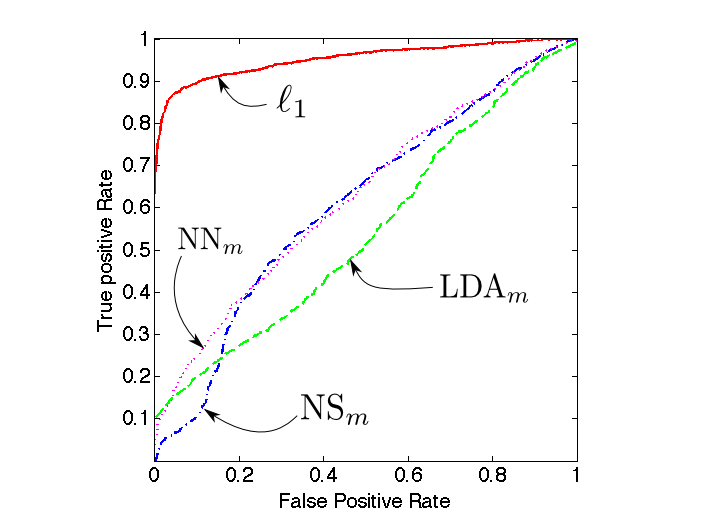
\includegraphics[width=5in]{figures_cvpr/roc3.png} 
}
\caption{{\bf Large-scale experiments on Multi PIE.} {\bf Top:} Recognition rates; {\bf Bottom:} ROC curves for our algorithm (labeled as ``$\ell_1$''), compared with those for NN$_m$, NS$_m$, and LDA$_m$.} \label{tab:multipie}
\end{figure}

\paragraph{Cause of errors.} Our algorithm's errors are mostly caused by a few subjects who significantly change their appearances between sessions (such as hair, facial hair, and eyeglasses). Some representative examples are shown in Figure \ref{fig:failed-examples}. In fact, for those subjects, alignment and recognition fail on almost all test illuminations.\vspace{0mm} %This may be due the limited number of illuminations present in the training. \vspace{0mm}
\begin{figure}
\centering

\includegraphics[scale=0.4,clip=true]{figures_cvpr/079_01_01_051_08.png} 
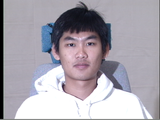
\includegraphics[scale=0.4,clip=true]{figures_cvpr/130_01_01_051_08.png} 
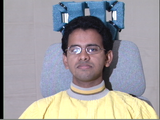
\includegraphics[scale=0.4,clip=true]{figures_cvpr/163_01_01_051_08.png} 
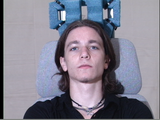
\includegraphics[scale=0.4,clip=true]{figures_cvpr/175_01_01_051_08.png} 

\includegraphics[scale=0.4,clip=true]{figures_cvpr/118_01_01_051_08.png} 

\includegraphics[scale=0.4,clip=true]{figures_cvpr/223_01_01_051_08.png} \\

\includegraphics[scale=0.4,clip=true]{figures_cvpr/079_02_01_051_08.png} 
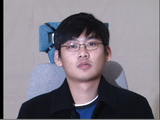
\includegraphics[scale=0.4,clip=true]{figures_cvpr/130_02_01_051_08.png} 

\includegraphics[scale=0.4,clip=true]{figures_cvpr/163_02_01_051_08.png} 

\includegraphics[scale=0.4,clip=true]{figures_cvpr/175_02_01_051_08.png} 
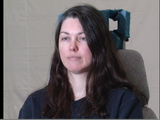
\includegraphics[scale=0.4,clip=true]{figures_cvpr/118_02_01_140_08.png} 
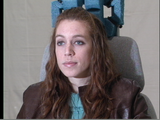
\includegraphics[scale=0.4,clip=true]{figures_cvpr/223_02_01_140_08.png} 
\caption{{\bf Representative examples of failed Multi-PIE subjects}. {\bf Top:} training from Session 1; {\bf Bottom:} test images from Session 2 -- first four are frontal and the last two with $15^\circ$ pose. Notice the change of hair style and facial hair, which makes alignment fail on those subjects, actually regardless of test image illuminations.\vspace{0mm}}\label{fig:failed-examples}
\end{figure}

\paragraph{Pose and expression.} We also run limited tests of our algorithm on images with pose and expression in Multi-PIE.  Using the same training as above, we test our algorithm on images in Session 2 with $15^\circ$ pose, for all 20 illuminations. The recognition rate is 77.5\%. We also test our algorithm on images in Session 3 with smile. For illumination 0 (ambient), the rate is 58.5\%, for illumination 10, the rate is 68.6\%.\vspace{0mm}


\subsection{Tests on our own datasets}\label{sec:own-data}\vspace{0mm}
Using the training acquisition system that we have described in the previous section, Figure \ref{fig:system}, we have collected the frontal view of 74 subjects {\em without eyeglasses} under 38 illuminations shown in Figure \ref{fig:illumination-patterns}. For testing our algorithm, we have also taken 593 images of these subjects with a different camera under a variety of practical conditions.\vspace{0mm}

\paragraph{Limitation of frontal illuminations.}
To see how training illuminations affect the performance of our algorithm in practice, we now compare how well a few frontal illuminations can interpolate: 1. other frontal illuminations taken under the same laboratory conditions, and 2. typical indoor and outdoor illuminations. To this end, we select 20 subjects from the face database acquired by our system and use 7 illuminations per subject as training. The illuminations are chosen to be similar to the 7 illuminations used in the previous experiment on Multi-PIE.\footnote{We use the illumination set $\{6, 9, 12, 13, 18, 21, 22\}$ shown in Figure \ref{fig:illumination-patterns}(b) to mimic the illumination set $\{0, 1, 6, 7, 13, 14, 18\}$ in Multi-PIE.} We then test our algorithm on the remaining $24 - 7 = 17$ frontal illuminations for all the 20 subjects. The recognition rate is $99.7\%$, nearly perfect. We also test our algorithm on $173$ frontal images of these subjects taken under a variety of indoor and outdoor conditions (in category 1 specified below), similar to the one shown in Figure \ref{fig:promo}, and the recognition drops down to $93.6\%$. One would expect the rate to drop even further when the number of subjects increases.\vspace{0mm}

\paragraph{Large-scale test with sufficient training illuminations.}
Now we use all 74 subjects and 38 illuminations in the training and test on 593 images taken under a variety of conditions. Based on the main variability in the test images, we have partitioned them into five main categories:%\vspace{0mm}
\begin{small}
\begin{description}
\item[C1:] 242 images of 47 subjects without eyeglasses, generally frontal view, under a variety of practical illuminations (indoor and outdoor) (Fig. 10, row 1). %\vspace{0mm}
\item[C2:] 109 images of 23 subjects with eyeglasses (Fig. 10, row 2).%\vspace{0mm}
\item[C3:] 19 images of 14 subjects with sunglasses (Fig. 10, row 3).%\vspace{0mm}
\item[C4:] 100 images of 40 subjects with noticeable expressions, poses, mild blur, and sometimes occlusion (Fig. 11, both rows).%\vspace{0mm}
\item[C5:] 123 images of 17 subjects with little control (out of focus, motion blur, significant pose, large occlusion, funny faces, extreme expressions) (Fig. 12, both rows).%\vspace{0mm}
\end{description}
\end{small}
We apply Viola and Jones' face detector on these images and directly use the detected faces as the input to our algorithm. The table below reports the performance of our algorithm on each category. The errors include failures of the face detector on some of the more challenging images.\vspace{0mm}
\begin{table}[h]	
\centering
\begin{tabular}{|l|c|c|c|c|c| }
\hline
Test Categories & C1 & C2 & C3 & C4 & C5  \\
\hline
\hline
Rec. Rates (\%) &  95.9 & 91.5 & 63.2 & 73.7 & 53.5 \\
\hline
\end{tabular} \vspace{0mm}
\end{table}

\begin{figure}
\centering

\includegraphics[scale=0.35,clip=true]{figures_cvpr/examples/1/DSC_1319.jpg} 
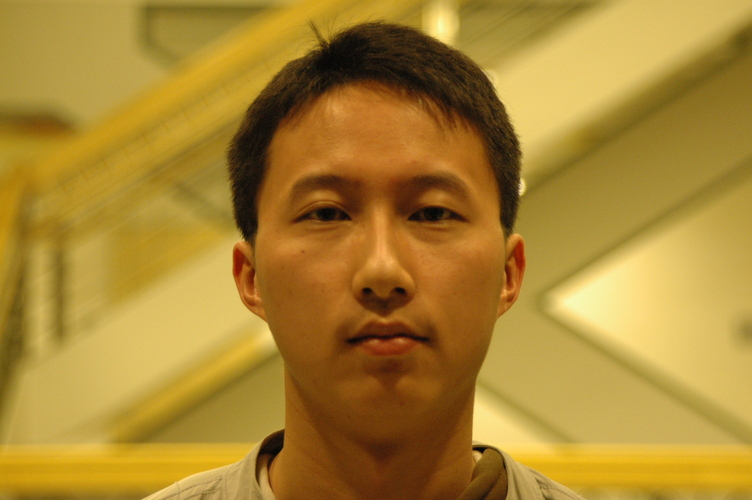
\includegraphics[scale=0.35,clip=true]{figures_cvpr/examples/1/DSC_1531.jpg} 

\includegraphics[scale=0.35,clip=true]{figures_cvpr/examples/1/DSC_1574.jpg} 
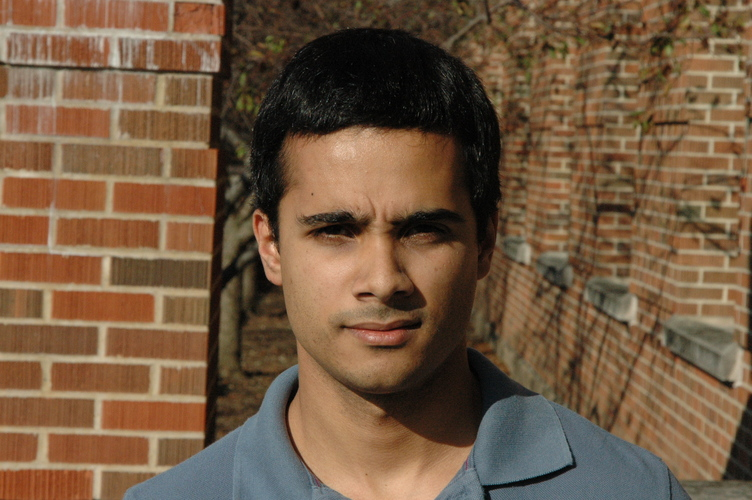
\includegraphics[scale=0.35,clip=true]{figures_cvpr/examples/1/DSC_1622.jpg} 
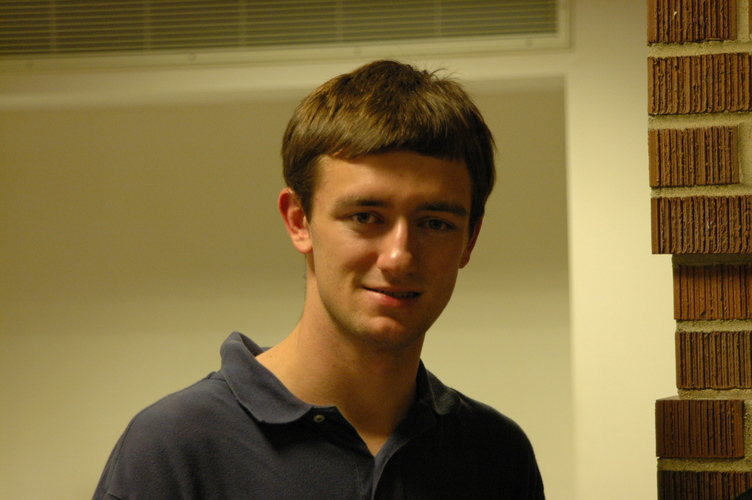
\includegraphics[scale=0.35,clip=true]{figures_cvpr/examples/1/DSC_1786.jpg} \\
\includegraphics[scale=0.35,clip=true]{figures_cvpr/examples/2/DSC_1448.jpg} 
\includegraphics[scale=0.35,clip=true]{figures_cvpr/examples/2/DSC_1585.jpg} 
\includegraphics[scale=0.35,clip=true]{figures_cvpr/examples/2/DSC_1588.jpg} 
\includegraphics[scale=0.35,clip=true]{figures_cvpr/examples/2/DSC_1666.jpg} 
\includegraphics[scale=0.35,clip=true]{figures_cvpr/examples/2/DSC_1874.jpg} \\
\includegraphics[scale=0.35,clip=true]{figures_cvpr/examples/3/DSC_1572.jpg} 
\includegraphics[scale=0.35,clip=true]{figures_cvpr/examples/3/DSC_1587.jpg} 
\includegraphics[scale=0.35,clip=true]{figures_cvpr/examples/3/DSC_1623.jpg} 
\includegraphics[scale=0.35,clip=true]{figures_cvpr/examples/3/DSC_1652.jpg} 
\includegraphics[scale=0.35,clip=true]{figures_cvpr/examples/3/DSC_1675.jpg} 
 \caption{{\bf Representative examples of categories 1-3}. One row for each category.\vspace{0mm}}\label{fig:examples1-3}
%\end{figure}
%\begin{figure}
\centering
\includegraphics[scale=0.35,clip=true]{figures_cvpr/examples/4/success/DSC_1579.jpg} 
\includegraphics[scale=0.35,clip=true]{figures_cvpr/examples/4/success/DSC_1839.jpg} 
\includegraphics[scale=0.35,clip=true]{figures_cvpr/examples/4/success/DSC_1883.jpg} 
\includegraphics[scale=0.35,clip=true]{figures_cvpr/examples/4/success/DSC_1922.jpg} 
\includegraphics[scale=0.35,clip=true]{figures_cvpr/examples/4/success/DSC_2000.jpg} \\
\includegraphics[scale=0.35,clip=true]{figures_cvpr/examples/4/failure/DSC_1568.jpg} 
\includegraphics[scale=0.35,clip=true]{figures_cvpr/examples/4/failure/DSC_1578.jpg} 
\includegraphics[scale=0.35,clip=true]{figures_cvpr/examples/4/failure/DSC_1500.jpg} 
\includegraphics[scale=0.35,clip=true]{figures_cvpr/examples/4/failure/DSC_1930.jpg} 
\includegraphics[scale=0.35,clip=true]{figures_cvpr/examples/4/failure/DSC_1985.jpg} 
 \caption{{\bf Representative examples of category 4}. Top row: successful examples. Bottom row: failures.}\label{fig:examples4}
\vspace{0mm}
\centering
\includegraphics[scale=0.35,clip=true]{figures_cvpr/examples/5/success/DSC_1664.jpg} 
\includegraphics[scale=0.35,clip=true]{figures_cvpr/examples/5/success/DSC_1777.jpg} 
\includegraphics[scale=0.35,clip=true]{figures_cvpr/examples/5/success/DSC_1871.jpg} 
\includegraphics[scale=0.35,clip=true]{figures_cvpr/examples/5/success/DSC_1913.jpg} 
\includegraphics[scale=0.35,clip=true]{figures_cvpr/examples/5/success/DSC_2005.jpg} \\
\includegraphics[scale=0.35,clip=true]{figures_cvpr/examples/5/failure/DSC_1669.jpg} 
\includegraphics[scale=0.35,clip=true]{figures_cvpr/examples/5/failure/DSC_1800.jpg} 
\includegraphics[scale=0.35,clip=true]{figures_cvpr/examples/5/failure/DSC_1870.jpg} 
\includegraphics[scale=0.35,clip=true]{figures_cvpr/examples/5/failure/DSC_1917.jpg} 
\includegraphics[scale=0.35,clip=true]{figures_cvpr/examples/5/failure/DSC_2008.jpg} 
 \caption{{\bf Representative examples of category 5}. Top row: successful examples. Bottom row: failures.\vspace{0mm}}\label{fig:examples5}
\end{figure}

\vspace{0mm}
\section{Conclusion}\vspace{0mm}
We have proposed a new algorithm and system for recognizing human faces from images taken under practical conditions. The proposed system is very {\em simple} and hence the results are easy to reproduce. The proposed algorithm is {\em scalable} both in terms of computational complexity and recognition performance. The system is directly compatible with off-the-shelf face detectors and achieves extremely {\em stable} performance under a wide range of variations in illumination, misalignment, pose, and occlusion. We achieve very good recognition performance on large-scale tests with public datasets and our practical face images, using only frontal 2D images in the training without any explicit 3D face model. 
%Our implementation still has plenty of room for further engineering improvements.\vspace{0mm}

%
%{\small
%\bibliographystyle{ieee}
%\bibliography{cvpr09_faces}
%}

%\end{document}

